%==============================================================================
% EECS 127 - Lecture 2: Linear Algebra Review - Vector Norms
%==============================================================================

\documentclass[10pt, twocolumn]{article}
\usepackage[margin=0.75in, columnsep=0.3in]{geometry}

%------------------------------------------------------------------------------
% REQUIRED PACKAGES
%------------------------------------------------------------------------------
\usepackage{amsmath, amssymb, amsthm}
\usepackage{microtype}
\usepackage{enumitem}
\usepackage{fancyhdr}
\usepackage{titlesec}
\usepackage{tcolorbox}
\usepackage{booktabs}
\usepackage{tikz}
\usetikzlibrary{positioning, arrows.meta, calc, shapes.geometric}
\usetikzlibrary{decorations.pathreplacing}

%------------------------------------------------------------------------------
% SPACING
%------------------------------------------------------------------------------
\linespread{1.18}
\setlength{\parskip}{0.8ex plus 0.3ex minus 0.1ex}
\setlength{\abovedisplayskip}{8pt plus 3pt minus 3pt}
\setlength{\belowdisplayskip}{8pt plus 3pt minus 3pt}
\setlength{\abovedisplayshortskip}{4pt plus 2pt}
\setlength{\belowdisplayshortskip}{4pt plus 2pt}

%------------------------------------------------------------------------------
% BOX STYLES
%------------------------------------------------------------------------------
\tcbset{
    boxrule=0.8pt,
    colback=white,
    colframe=black,
    arc=0pt,
    boxsep=4pt,
    left=5pt, right=5pt, top=6pt, bottom=6pt,
    before skip=8pt, after skip=8pt
}

\newtcolorbox{result}{
    boxrule=0pt,
    colback=black!5,
    colframe=white,
    arc=0pt,
    boxsep=3pt,
    left=5pt, right=5pt, top=6pt, bottom=6pt,
    before skip=8pt, after skip=8pt
}

%------------------------------------------------------------------------------
% SECTION FORMATTING
%------------------------------------------------------------------------------
\titleformat{\section}{\large\bfseries}{\thesection.}{0.5em}{}
\titleformat{\subsection}{\normalsize\bfseries}{\thesubsection}{0.5em}{}
\titlespacing*{\section}{0pt}{2.5ex plus 0.5ex}{1.5ex plus 0.3ex}
\titlespacing*{\subsection}{0pt}{2.0ex plus 0.4ex}{1.0ex plus 0.2ex}

%------------------------------------------------------------------------------
% LIST FORMATTING
%------------------------------------------------------------------------------
\setlist{itemsep=3pt, topsep=6pt, parsep=2pt, leftmargin=1.5em}

%------------------------------------------------------------------------------
% HEADER/FOOTER
%------------------------------------------------------------------------------
\pagestyle{fancy}
\fancyhf{}
\fancyhead[L]{\small EECS 127}
\fancyhead[R]{\small Lecture 2}
\fancyfoot[C]{\small\thepage}
\renewcommand{\headrulewidth}{0.4pt}

%------------------------------------------------------------------------------
% THEOREM ENVIRONMENTS
%------------------------------------------------------------------------------
\theoremstyle{definition}
\newtheorem{definition}{Definition}
\newtheorem{example}{Example}

\theoremstyle{plain}
\newtheorem{theorem}{Theorem}
\newtheorem{lemma}[theorem]{Lemma}
\newtheorem{claim}{Claim}

%------------------------------------------------------------------------------
% CUSTOM COMMANDS
%------------------------------------------------------------------------------
\newcommand{\RR}{\mathbb{R}}
\newcommand{\NN}{\mathcal{N}}
\newcommand{\Range}{\mathcal{R}}
\DeclareMathOperator{\rank}{rank}
\DeclareMathOperator{\spn}{span}
\DeclareMathOperator{\argmax}{argmax}
\DeclareMathOperator{\sign}{sign}

%==============================================================================

\begin{document}

\noindent
\begin{minipage}{\linewidth}
    \centering
    \textbf{\Large Lecture 2: Linear Algebra Review - Vector Norms} \\[0.5em]
    \hrule
\end{minipage}
\vspace{1em}

%==============================================================================
\section{Vector Norms}
%==============================================================================

We begin with the most basic way to measure the ``size'' of a vector.

The standard \textbf{Euclidean norm} (or \textbf{2-norm}) of a vector $\vec{x} \in \RR^n$ is:
\[
    \|\vec{x}\| = \sqrt{\sum_{i=1}^{n} x_i^2}
\]

This is a special case of a more general concept.

%------------------------------------------------------------------------------
\subsection{Definition of a Norm}
%------------------------------------------------------------------------------

\begin{tcolorbox}
\begin{definition}[Norm]
A function $\|\cdot\|: X \to \RR$ is a \textbf{norm} if it satisfies three properties for all $\vec{x}, \vec{y} \in X$ and all $\alpha \in \RR$:
\begin{enumerate}
    \item \textbf{Non-negativity:} $\|\vec{x}\| \ge 0$, and $\|\vec{x}\| = 0$ if and only if $\vec{x} = \vec{0}$
    \item \textbf{Triangle inequality:} $\|\vec{x} + \vec{y}\| \le \|\vec{x}\| + \|\vec{y}\|$
    \item \textbf{Absolute homogeneity:} $\|\alpha \vec{x}\| = |\alpha| \, \|\vec{x}\|$
\end{enumerate}
\end{definition}
\end{tcolorbox}

These axioms capture our intuition about ``length'': it is always non-negative, the direct path is never longer than a detour, and scaling a vector scales its length proportionally.

\begin{center}
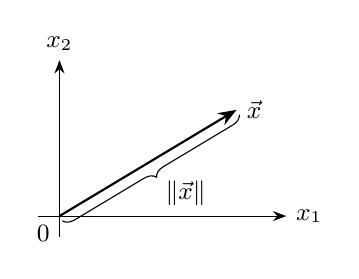
\begin{tikzpicture}[scale=0.9, >=Stealth]
    % Axes
    \draw[->] (-0.3,0) -- (3.2,0) node[right] {\small $x_1$};
    \draw[->] (0,-0.3) -- (0,2.2) node[above] {\small $x_2$};
    % Vector
    \draw[->, thick] (0,0) -- (2.5,1.5) node[right] {\small $\vec{x}$};
    % Norm label with brace
    \draw[decorate, decoration={brace, amplitude=4pt, mirror, raise=2pt}] (0,0) -- (2.5,1.5) node[midway, below right=4pt] {\small $\|\vec{x}\|$};
    % Origin label
    \node[below left] at (0,0) {\small $0$};
\end{tikzpicture}
\end{center}

\textbf{Why each axiom matters.}
\textbf{Positive definiteness} (the ``if and only if'' part of non-negativity) prevents any nonzero vector from having zero size; without it, distinct vectors could be indistinguishable.
\textbf{Homogeneity} says that scaling a vector by $\alpha$ scales its size by $|\alpha|$, so the norm is compatible with the linear structure of the space.
\textbf{The triangle inequality} encodes the geometry we need for bounding errors, proving convergence of iterative algorithms, and establishing stability of solutions under perturbation.

\begin{example}[Verifying the norm axioms for $\ell_2$]
Let $\vec{x} = (1, -2)^\top$ and $\vec{y} = (2, 1)^\top$. We verify all three axioms for the $\ell_2$ norm.

\textbf{Positive definiteness.} Since $\vec{x} \ne \vec{0}$, we need $\|\vec{x}\|_2 > 0$:
\[
    \|\vec{x}\|_2 = \sqrt{1^2 + (-2)^2} = \sqrt{5} > 0 \quad \checkmark
\]

\textbf{Homogeneity.} Take $\alpha = -3$. We check $\|\alpha \vec{x}\|_2 = |\alpha| \, \|\vec{x}\|_2$:
\[
    \alpha \vec{x} = (-3, 6)^\top, \quad
    \|\alpha \vec{x}\|_2 = \sqrt{9 + 36} = 3\sqrt{5} = |-3| \cdot \sqrt{5} \quad \checkmark
\]

\textbf{Triangle inequality.} We check $\|\vec{x} + \vec{y}\|_2 \le \|\vec{x}\|_2 + \|\vec{y}\|_2$:
\[
    \vec{x} + \vec{y} = (3, -1)^\top, \quad \|\vec{x} + \vec{y}\|_2 = \sqrt{10}, \quad \|\vec{y}\|_2 = \sqrt{5}
\]
\begin{result}
\[
    \|\vec{x} + \vec{y}\|_2 = \sqrt{10} \approx 3.16 \le 2\sqrt{5} \approx 4.47 = \|\vec{x}\|_2 + \|\vec{y}\|_2 \quad \checkmark
\]
\end{result}
\end{example}

%------------------------------------------------------------------------------
\subsection{The $\ell_p$ Norm}
%------------------------------------------------------------------------------

The most important family of norms is the \textbf{$\ell_p$ norm}, parameterized by $p$.

\begin{tcolorbox}
\begin{definition}[$\ell_p$ Norm]
For $1 \le p < \infty$, the $\ell_p$ norm of $\vec{x} \in \RR^n$ is:
\[
    \|\vec{x}\|_p = \left(\sum_{i=1}^{n} |x_i|^p\right)^{1/p}
\]
\end{definition}
\end{tcolorbox}

Different values of $p$ give different norms, each emphasizing a different notion of size: $\|\vec{x}\|_1$ measures the total magnitude across all components, $\|\vec{x}\|_2$ measures the Euclidean length, and $\|\vec{x}\|_\infty$ measures the largest coordinate in absolute value.

\textbf{$p = 2$: Euclidean norm.} The familiar geometric distance:
\begin{result}
\[
    \|\vec{x}\|_2 = \sqrt{\sum_{i=1}^{n} x_i^2} = \sqrt{\vec{x}^\top \vec{x}}
\]
\end{result}

\textbf{$p = 1$: Manhattan norm.} The sum of absolute values:
\begin{result}
\[
    \|\vec{x}\|_1 = \sum_{i=1}^{n} |x_i|
\]
\end{result}

This measures distance along axis-aligned paths (like walking on a grid of city blocks).

\begin{example}[Comparing norms on a single vector]
Let $\vec{x} = (3, -4)^\top$. The three standard $\ell_p$ norms give different values:
\[
    \|\vec{x}\|_1 = |3| + |-4| = 7, \qquad
    \|\vec{x}\|_2 = \sqrt{9 + 16} = 5, \qquad
    \|\vec{x}\|_\infty = \max(3, 4) = 4
\]
\begin{result}
\[
    \|\vec{x}\|_\infty = 4 \;\le\; \|\vec{x}\|_2 = 5 \;\le\; \|\vec{x}\|_1 = 7
\]
\end{result}
The ordering $\|\vec{x}\|_\infty \le \|\vec{x}\|_2 \le \|\vec{x}\|_1$ holds for every $\vec{x} \in \RR^n$.
\end{example}

\textbf{$p = \infty$: Max norm.} The largest absolute component:
\begin{result}
\[
    \|\vec{x}\|_\infty = \max_{i = 1, 2, \ldots, n} |x_i|
\]
\end{result}

This is the limiting case as $p \to \infty$. Only the largest component matters.

%------------------------------------------------------------------------------
\subsection{The $\ell^\infty$ Norm as a Limit}
%------------------------------------------------------------------------------

The $\ell_\infty$ norm is not just a separate definition---it arises naturally as the limit of $\ell_p$ norms.

\begin{tcolorbox}
\begin{claim}
For any $\vec{x} \in \RR^n$, $\|\vec{x}\|_\infty = \lim_{p \to \infty} \|\vec{x}\|_p$.
\end{claim}
\end{tcolorbox}

\begin{proof}
Let $M = \max_{i} |x_i| = \|\vec{x}\|_\infty$. We use a squeeze argument.

\textbf{Lower bound.} The sum includes a term equal to $M^p$, so $\|\vec{x}\|_p \ge (M^p)^{1/p} = M$.

\textbf{Upper bound.} Since $|x_i| \le M$ for every $i$, we have $\|\vec{x}\|_p \le (nM^p)^{1/p} = n^{1/p} M$.

\textbf{Squeeze.} Combining:
\begin{result}
\[
    M \;\le\; \|\vec{x}\|_p \;\le\; n^{1/p} \cdot M
\]
\end{result}
As $p \to \infty$, $n^{1/p} \to 1$, so both sides converge to $M = \|\vec{x}\|_\infty$.
\end{proof}

\begin{example}[Convergence of $\|\vec{x}\|_p$ to $\|\vec{x}\|_\infty$]
Let $\vec{x} = (1, 2)^\top$, so $\|\vec{x}\|_\infty = 2$.

\begin{center}
\begin{tabular}{ccl}
\toprule
$p$ & $\|\vec{x}\|_p$ & Value \\
\midrule
$1$ & $|1| + |2|$ & $3.000$ \\
$2$ & $\sqrt{1 + 4}$ & $2.236$ \\
$4$ & $(1 + 16)^{1/4}$ & $2.031$ \\
$10$ & $(1 + 1024)^{1/10}$ & $2.003$ \\
$\infty$ & $\max(1, 2)$ & $2.000$ \\
\bottomrule
\end{tabular}
\end{center}

As $p$ increases, $\|\vec{x}\|_p$ decreases monotonically toward $\|\vec{x}\|_\infty = 2$.
\end{example}

\begin{tcolorbox}[colframe=black!50]
\textbf{Rigor note:} For $0 < p < 1$, the formula $\left(\sum_{i} |x_i|^p\right)^{1/p}$ does \emph{not} define a norm because the triangle inequality fails. For example, with $p = 1/2$ and $\vec{e}_1, \vec{e}_2 \in \RR^2$:
\[
    \|\vec{e}_1 + \vec{e}_2\|_{1/2} = (1 + 1)^{2} = 4 > 2 = \|\vec{e}_1\|_{1/2} + \|\vec{e}_2\|_{1/2}
\]
This is why we require $p \ge 1$.
\end{tcolorbox}

%==============================================================================
\section{Inner Product Inequalities}
%==============================================================================

%------------------------------------------------------------------------------
\subsection{Cauchy--Schwarz Inequality}
%------------------------------------------------------------------------------

The most fundamental inequality relating inner products and norms:

\begin{tcolorbox}
\begin{theorem}[Cauchy--Schwarz Inequality]
For all $\vec{x}, \vec{y} \in \RR^n$:
\[
    |\vec{x}^\top \vec{y}| \le \|\vec{x}\|_2 \, \|\vec{y}\|_2
\]
with equality if and only if $\vec{x}$ and $\vec{y}$ are linearly dependent.
\end{theorem}
\end{tcolorbox}

\begin{center}
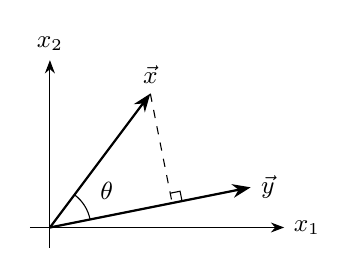
\begin{tikzpicture}[scale=0.85, >=Stealth]
    \draw[->] (-0.3,0) -- (3.5,0) node[right] {\small $x_1$};
    \draw[->] (0,-0.3) -- (0,2.5) node[above] {\small $x_2$};
    % Vector y
    \draw[->, thick] (0,0) -- (3,0.6) node[right] {\small $\vec{y}$};
    % Vector x
    \draw[->, thick] (0,0) -- (1.5,2) node[above] {\small $\vec{x}$};
    % Projection of x onto y
    \coordinate (P) at (1.827, 0.365);
    \draw[dashed, thin] (1.5,2) -- (P);
    % Right-angle marker at P (size 0.15)
    % y-dir unit: (0.9806, 0.1961), perp unit: (-0.1961, 0.9806)
    \coordinate (Ra) at ($(P) + 0.15*(-0.1961, 0.9806)$);
    \coordinate (Rb) at ($(P) + 0.15*(-0.1961, 0.9806) + 0.15*(0.9806, 0.1961)$);
    \coordinate (Rc) at ($(P) + 0.15*(0.9806, 0.1961)$);
    \draw[thin] (Ra) -- (Rb) -- (Rc);
    % Angle arc
    \draw (0.6,0.12) arc[start angle=11.3, end angle=53.1, radius=0.61];
    \node at (0.85, 0.55) {\small $\theta$};
\end{tikzpicture}
\end{center}

\begin{proof}
If $\vec{y} = \vec{0}$, both sides are zero and the inequality holds trivially. So assume $\vec{y} \ne \vec{0}$. For any $t \in \RR$, the squared norm is non-negative:
\[
    0 \le \|\vec{x} - t\vec{y}\|_2^2 = (\vec{x} - t\vec{y})^\top(\vec{x} - t\vec{y}) = \|\vec{x}\|_2^2 - 2t(\vec{x}^\top \vec{y}) + t^2 \|\vec{y}\|_2^2
\]
The right-hand side is a quadratic in $t$ that is non-negative for all $t \in \RR$. A quadratic $At^2 + Bt + C \ge 0$ for all $t$ if and only if its discriminant satisfies $B^2 - 4AC \le 0$. Here $A = \|\vec{y}\|_2^2$, $B = -2(\vec{x}^\top \vec{y})$, and $C = \|\vec{x}\|_2^2$, so:
\[
    \bigl(-2(\vec{x}^\top \vec{y})\bigr)^2 - 4\|\vec{y}\|_2^2 \|\vec{x}\|_2^2 \le 0
\]
\[
    4(\vec{x}^\top \vec{y})^2 \le 4\|\vec{x}\|_2^2 \|\vec{y}\|_2^2
\]
Dividing by 4 gives $(\vec{x}^\top \vec{y})^2 \le \|\vec{x}\|_2^2 \, \|\vec{y}\|_2^2$. Taking square roots:
\begin{result}
\[
    |\vec{x}^\top \vec{y}| \le \|\vec{x}\|_2 \, \|\vec{y}\|_2
\]
\end{result}
\end{proof}

\textbf{Equality condition.} Equality holds if and only if $\vec{x}$ and $\vec{y}$ are linearly dependent, i.e., one is a scalar multiple of the other. This is because the discriminant equals zero precisely when $\|\vec{x} - t\vec{y}\|_2^2 = 0$ for some $t$, meaning $\vec{x} = t\vec{y}$.

\begin{example}[Cauchy--Schwarz with specific vectors]
Let $\vec{x} = (1, 2)^\top$ and $\vec{y} = (3, -1)^\top$. We compute:
\[
    \vec{x}^\top \vec{y} = (1)(3) + (2)(-1) = 1
\]
\[
    \|\vec{x}\|_2 = \sqrt{1^2 + 2^2} = \sqrt{5}, \qquad \|\vec{y}\|_2 = \sqrt{3^2 + (-1)^2} = \sqrt{10}
\]
The inequality gives:
\[
    |\vec{x}^\top \vec{y}| = 1 \le \sqrt{5} \cdot \sqrt{10} = \sqrt{50} \approx 7.07
\]
Equality does \emph{not} hold here, since $\vec{x}$ and $\vec{y}$ are not scalar multiples of each other (there is no $\alpha$ with $(1, 2)^\top = \alpha(3, -1)^\top$).
\end{example}

Cauchy--Schwarz says that the inner product of two vectors is bounded by the product of their lengths. This is the algebraic version of the geometric fact that $|\cos\theta| \le 1$.

%------------------------------------------------------------------------------
\subsection{H\"{o}lder's Inequality}
%------------------------------------------------------------------------------

Cauchy--Schwarz is a special case of a more general result.

\begin{tcolorbox}
\begin{theorem}[H\"{o}lder's Inequality]
Let $\vec{x}, \vec{y} \in \RR^n$ and let $p, q \ge 1$ satisfy $\frac{1}{p} + \frac{1}{q} = 1$. Then:
\[
    |\vec{x}^\top \vec{y}| \le \|\vec{x}\|_p \, \|\vec{y}\|_q
\]
\end{theorem}
\end{tcolorbox}

The pair $(p, q)$ satisfying $\frac{1}{p} + \frac{1}{q} = 1$ are called \textbf{conjugate exponents}. Important cases:

\begin{itemize}
    \item $p = q = 2$: recovers Cauchy--Schwarz
    \item $p = 1, q = \infty$: gives $|\vec{x}^\top \vec{y}| \le \|\vec{x}\|_1 \, \|\vec{y}\|_\infty$
    \item $p = \infty, q = 1$: gives $|\vec{x}^\top \vec{y}| \le \|\vec{x}\|_\infty \, \|\vec{y}\|_1$
\end{itemize}

\begin{example}[H\"{o}lder with $p = 1$, $q = \infty$]
Let $\vec{x} = (1, -1, 0)^\top$ and $\vec{y} = (4, -4, 2)^\top$. We compute:
\[
    \sum_{i=1}^{3} |x_i y_i| = |1 \cdot 4| + |(-1)(-4)| + |0 \cdot 2| = 4 + 4 + 0 = 8
\]
\[
    \|\vec{x}\|_1 = |1| + |-1| + |0| = 2, \qquad \|\vec{y}\|_\infty = \max(|4|, |-4|, |2|) = 4
\]
So $|\vec{x}^\top \vec{y}| = 8 = 2 \cdot 4 = \|\vec{x}\|_1 \, \|\vec{y}\|_\infty$. This is an equality case: the bound is tight because each nonzero $x_i$ is paired with a $y_i$ achieving the maximum absolute value.
\end{example}

%------------------------------------------------------------------------------
\subsubsection*{Proof of H\"{o}lder's Inequality}
%------------------------------------------------------------------------------

We prove the three cases separately.

\textbf{Endpoint case $p = 1$, $q = \infty$.}

\begin{proof}
By the triangle inequality for sums and the definition of the $\ell_\infty$ norm:
\[
    |\vec{x}^\top \vec{y}| = \left|\sum_{i=1}^{n} x_i y_i\right| \le \sum_{i=1}^{n} |x_i y_i| = \sum_{i=1}^{n} |x_i| |y_i|
\]
Since $|y_i| \le \max_j |y_j| = \|\vec{y}\|_\infty$ for every $i$, we can bound:
\[
    \sum_{i=1}^{n} |x_i| |y_i| \le \|\vec{y}\|_\infty \sum_{i=1}^{n} |x_i| = \|\vec{x}\|_1 \, \|\vec{y}\|_\infty
\]
Combining the two chains:
\begin{result}
\[
    |\vec{x}^\top \vec{y}| \le \sum_{i=1}^{n} |x_i| |y_i| \le \left(\max_i |y_i|\right) \sum_{i=1}^{n} |x_i| = \|\vec{x}\|_1 \, \|\vec{y}\|_\infty
\]
\end{result}
\end{proof}

\textbf{Endpoint case $p = \infty$, $q = 1$.}

\begin{proof}
The argument is symmetric. We have:
\[
    |\vec{x}^\top \vec{y}| \le \sum_{i=1}^{n} |x_i| |y_i| \le \left(\max_i |x_i|\right) \sum_{i=1}^{n} |y_i| = \|\vec{x}\|_\infty \, \|\vec{y}\|_1
\]
\end{proof}

\textbf{General case $1 < p < \infty$.}

The proof relies on a classical pointwise inequality.

\begin{tcolorbox}
\begin{lemma}[Young's Inequality]
For $a, b \ge 0$ and conjugate exponents $p, q > 1$ with $\frac{1}{p} + \frac{1}{q} = 1$:
\[
    ab \le \frac{a^p}{p} + \frac{b^q}{q}
\]
\end{lemma}
\end{tcolorbox}

Young's inequality follows from the concavity of the logarithm: $\log(ab) = \frac{1}{p}\log(a^p) + \frac{1}{q}\log(b^q) \le \log\!\left(\frac{a^p}{p} + \frac{b^q}{q}\right)$.

\begin{proof}[Proof of H\"{o}lder's inequality for $1 < p < \infty$]
If $\|\vec{x}\|_p = 0$ or $\|\vec{y}\|_q = 0$, the inequality holds trivially (both sides are zero). So assume both norms are positive.

\textbf{Step 1: Normalize.} Define:
\[
    u_i = \frac{|x_i|}{\|\vec{x}\|_p}, \qquad v_i = \frac{|y_i|}{\|\vec{y}\|_q}
\]
By construction, the normalized vectors satisfy:
\begin{result}
\[
    \sum_{i=1}^{n} u_i^p = \frac{1}{\|\vec{x}\|_p^p} \sum_{i=1}^{n} |x_i|^p = 1, \qquad \sum_{i=1}^{n} v_i^q = \frac{1}{\|\vec{y}\|_q^q} \sum_{i=1}^{n} |y_i|^q = 1
\]
\end{result}

\textbf{Step 2: Apply Young's inequality.} For each $i = 1, \ldots, n$, apply Young's inequality to $a = u_i$ and $b = v_i$:
\[
    u_i \, v_i \le \frac{u_i^p}{p} + \frac{v_i^q}{q}
\]

\textbf{Step 3: Sum over all components.}
\[
    \sum_{i=1}^{n} u_i \, v_i \le \frac{1}{p} \sum_{i=1}^{n} u_i^p + \frac{1}{q} \sum_{i=1}^{n} v_i^q = \frac{1}{p} \cdot 1 + \frac{1}{q} \cdot 1 = \frac{1}{p} + \frac{1}{q} = 1
\]

\textbf{Step 4: Undo the normalization.} Substituting back:
\[
    \sum_{i=1}^{n} \frac{|x_i|}{\|\vec{x}\|_p} \cdot \frac{|y_i|}{\|\vec{y}\|_q} \le 1
\]
Multiplying both sides by $\|\vec{x}\|_p \, \|\vec{y}\|_q$:
\[
    \sum_{i=1}^{n} |x_i| |y_i| \le \|\vec{x}\|_p \, \|\vec{y}\|_q
\]
Finally, since $|\vec{x}^\top \vec{y}| \le \sum_{i=1}^{n} |x_i| |y_i|$, we conclude:
\begin{result}
\[
    |\vec{x}^\top \vec{y}| \le \|\vec{x}\|_p \, \|\vec{y}\|_q
\]
\end{result}
\end{proof}

%------------------------------------------------------------------------------
\subsection{Minkowski's Inequality}
%------------------------------------------------------------------------------

\begin{tcolorbox}
\begin{theorem}[Minkowski's Inequality]
For $1 \le p \le \infty$ and $\vec{u}, \vec{v} \in \RR^n$:
\[
    \|\vec{u} + \vec{v}\|_p \le \|\vec{u}\|_p + \|\vec{v}\|_p
\]
\end{theorem}
\end{tcolorbox}

This is the triangle inequality for $\ell_p$ norms. For $p = 1$ and $p = \infty$ it is straightforward. For $1 < p < \infty$ it follows from H\"{o}lder's inequality.

\begin{proof}[Proof sketch for $1 < p < \infty$]
We expand $\|\vec{u} + \vec{v}\|_p^p$ and apply the triangle inequality componentwise:
\[
    \|\vec{u} + \vec{v}\|_p^p = \sum_{i=1}^{n} |u_i + v_i|^p = \sum_{i=1}^{n} |u_i + v_i|^{p-1} |u_i + v_i|
\]
\[
    \le \sum_{i=1}^{n} |u_i| \, |u_i + v_i|^{p-1} + \sum_{i=1}^{n} |v_i| \, |u_i + v_i|^{p-1}
\]
Apply H\"{o}lder's inequality to each sum with exponents $p$ and $q = \frac{p}{p-1}$. Note that the vector with components $|u_i + v_i|^{p-1}$ has $\ell_q$ norm:
\[
    \left(\sum_{i=1}^{n} \bigl(|u_i + v_i|^{p-1}\bigr)^q\right)^{1/q} = \left(\sum_{i=1}^{n} |u_i + v_i|^p\right)^{1/q} = \|\vec{u} + \vec{v}\|_p^{p/q}
\]
since $(p-1)q = p$. Applying H\"{o}lder to both sums:
\[
    \|\vec{u} + \vec{v}\|_p^p \le \|\vec{u}\|_p \, \|\vec{u} + \vec{v}\|_p^{p/q} + \|\vec{v}\|_p \, \|\vec{u} + \vec{v}\|_p^{p/q}
\]
\[
    = \bigl(\|\vec{u}\|_p + \|\vec{v}\|_p\bigr) \|\vec{u} + \vec{v}\|_p^{p/q}
\]
If $\|\vec{u} + \vec{v}\|_p = 0$, the inequality holds trivially. Otherwise, divide both sides by $\|\vec{u} + \vec{v}\|_p^{p/q}$. Since $p - p/q = p(1 - 1/q) = p \cdot \frac{1}{p} = 1$:
\begin{result}
\[
    \|\vec{u} + \vec{v}\|_p \le \|\vec{u}\|_p + \|\vec{v}\|_p
\]
\end{result}
\end{proof}

\begin{tcolorbox}[colframe=black!50]
\textbf{Remark.} Minkowski's inequality proves that the $\ell_p$ formula from Definition 2 really does satisfy the norm axioms for all $p \ge 1$. Non-negativity and absolute homogeneity are immediate from the definition; the triangle inequality is the nontrivial property, and it is precisely Minkowski's inequality.
\end{tcolorbox}

%==============================================================================
\section{Norm Balls}
%==============================================================================

\begin{tcolorbox}
\begin{definition}[Norm Ball]
The \textbf{unit norm ball} in the $\ell_p$ norm is the set of all vectors with norm at most 1:
\[
    B_p = \{\vec{x} \in \RR^n : \|\vec{x}\|_p \le 1\}
\]
\end{definition}
\end{tcolorbox}

The shape of $B_p$ depends on $p$. In $\RR^2$:

\begin{center}
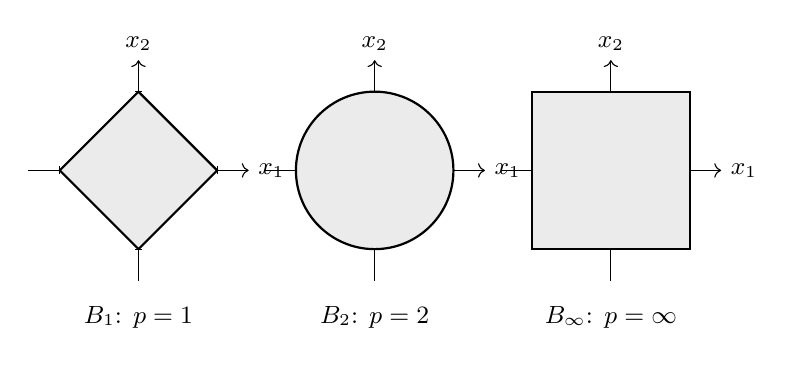
\begin{tikzpicture}[scale=1.0]
    % --- p = 1 (diamond) ---
    \begin{scope}[shift={(-3,0)}]
        \draw[->] (-1.4,0) -- (1.4,0) node[right] {\small $x_1$};
        \draw[->] (0,-1.4) -- (0,1.4) node[above] {\small $x_2$};
        \fill[black!8] (1,0) -- (0,1) -- (-1,0) -- (0,-1) -- cycle;
        \draw[thick] (1,0) -- (0,1) -- (-1,0) -- (0,-1) -- cycle;
        \foreach \x in {-1,1} {
            \draw (\x, 0.05) -- (\x, -0.05);
            \draw (0.05, \x) -- (-0.05, \x);
        }
        \node[below] at (0,-1.6) {\small $B_1$: $p = 1$};
    \end{scope}
    % --- p = 2 (circle) ---
    \begin{scope}[shift={(0,0)}]
        \draw[->] (-1.4,0) -- (1.4,0) node[right] {\small $x_1$};
        \draw[->] (0,-1.4) -- (0,1.4) node[above] {\small $x_2$};
        \fill[black!8] (0,0) circle (1);
        \draw[thick] (0,0) circle (1);
        \foreach \x in {-1,1} {
            \draw (\x, 0.05) -- (\x, -0.05);
            \draw (0.05, \x) -- (-0.05, \x);
        }
        \node[below] at (0,-1.6) {\small $B_2$: $p = 2$};
    \end{scope}
    % --- p = inf (square) ---
    \begin{scope}[shift={(3,0)}]
        \draw[->] (-1.4,0) -- (1.4,0) node[right] {\small $x_1$};
        \draw[->] (0,-1.4) -- (0,1.4) node[above] {\small $x_2$};
        \fill[black!8] (-1,-1) rectangle (1,1);
        \draw[thick] (-1,-1) rectangle (1,1);
        \foreach \x in {-1,1} {
            \draw (\x, 0.05) -- (\x, -0.05);
            \draw (0.05, \x) -- (-0.05, \x);
        }
        \node[below] at (0,-1.6) {\small $B_\infty$: $p = \infty$};
    \end{scope}
\end{tikzpicture}
\end{center}

\begin{itemize}
    \item $p = 2$: circle (all points at Euclidean distance $\le 1$)
    \item $p = 1$: diamond (constraint $|x_1| + |x_2| \le 1$)
    \item $p = \infty$: square (constraint $\max(|x_1|, |x_2|) \le 1$)
\end{itemize}

\begin{tcolorbox}[colframe=black!50]
\textbf{Key observation:} As $p$ increases from 1 to $\infty$, the norm ball ``inflates'' from a diamond through a circle to a square. Smaller $p$ produces ``spikier'' balls.
\end{tcolorbox}

%==============================================================================
\section{Optimization Over Norm Balls}
%==============================================================================

A natural question: given a fixed vector $\vec{y}$, what is the maximum inner product $\vec{x}^\top \vec{y}$ over all $\vec{x}$ in the unit $\ell_p$ ball?

\begin{result}
\[
    \max_{\|\vec{x}\|_p \le 1} \vec{x}^\top \vec{y}
\]
\end{result}

The answer depends on $p$ and reveals a deep connection between norms and their conjugates.

%------------------------------------------------------------------------------
\subsection{Upper Bound via H\"{o}lder}
%------------------------------------------------------------------------------

Before examining individual cases, we establish a universal upper bound.

For any $\vec{x}$ with $\|\vec{x}\|_p \le 1$, H\"{o}lder's inequality gives:
\[
    \vec{x}^\top \vec{y} \le |\vec{x}^\top \vec{y}| \le \|\vec{x}\|_p \, \|\vec{y}\|_q \le 1 \cdot \|\vec{y}\|_q = \|\vec{y}\|_q
\]
where $q$ is the conjugate exponent satisfying $\frac{1}{p} + \frac{1}{q} = 1$.

\begin{tcolorbox}[colframe=black!50]
\textbf{Upper bound:} $\displaystyle\max_{\|\vec{x}\|_p \le 1} \vec{x}^\top \vec{y} \le \|\vec{y}\|_q$ for \emph{every} $p \ge 1$.
\end{tcolorbox}

So the maximum is \emph{at most} $\|\vec{y}\|_q$. To show equality, it suffices to exhibit, for each $p$, a feasible $\vec{x}^\star$ with $\|\vec{x}^\star\|_p \le 1$ achieving $\vec{x}^{\star\top} \vec{y} = \|\vec{y}\|_q$.

%------------------------------------------------------------------------------
\subsection{Case $p = 2$: Euclidean Ball}
%------------------------------------------------------------------------------

\begin{example}[$p = 2$]
Maximize $\vec{x}^\top \vec{y}$ subject to $\|\vec{x}\|_2 \le 1$, with $\vec{y} = (1, 2)^\top$.
\end{example}

The inner product $\vec{x}^\top \vec{y}$ is maximized when $\vec{x}$ points in the same direction as $\vec{y}$. The optimal solution is:
\begin{result}
\[
    \vec{x}^\star = \frac{\vec{y}}{\|\vec{y}\|_2}
\]
\end{result}

\textbf{Verification.} We have $\|\vec{x}^\star\|_2 = 1$ (feasible), and:
\[
    \vec{x}^{\star\top} \vec{y} = \frac{\vec{y}^\top \vec{y}}{\|\vec{y}\|_2} = \frac{\|\vec{y}\|_2^2}{\|\vec{y}\|_2} = \|\vec{y}\|_2
\]

This matches the upper bound ($q = 2$ when $p = 2$), so $\vec{x}^\star$ is optimal.

\begin{tcolorbox}[colframe=black!50]
\textbf{Result:} $\displaystyle\max_{\|\vec{x}\|_2 \le 1} \vec{x}^\top \vec{y} = \|\vec{y}\|_2$. This is precisely Cauchy--Schwarz with equality.
\end{tcolorbox}

\textit{Geometrically: on the circle, the best point is the point in the direction of $\vec{y}$.}

\begin{center}
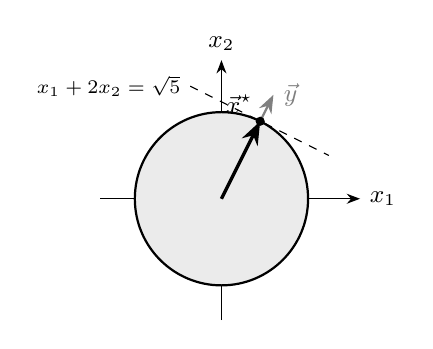
\begin{tikzpicture}[scale=1.1, >=Stealth]
    \draw[->] (-1.4,0) -- (1.6,0) node[right] {\small $x_1$};
    \draw[->] (0,-1.4) -- (0,1.6) node[above] {\small $x_2$};
    % Unit circle
    \fill[black!8] (0,0) circle (1);
    \draw[thick] (0,0) circle (1);
    % y vector (1,2), scaled to fit: show at (0.6, 1.2)
    \draw[->, thick, black!50] (0,0) -- (0.6,1.2) node[right] {\small $\vec{y}$};
    % x* = (1/sqrt5, 2/sqrt5) = (0.4472, 0.8944) on circle
    \coordinate (xstar) at (0.4472, 0.8944);
    \draw[->, very thick] (0,0) -- (xstar);
    \fill (xstar) circle (1.5pt) node[above left=-1pt] {\small $\vec{x}^\star$};
    % Tangent line: x1 + 2*x2 = sqrt(5) ≈ 2.236
    % At x2=0: x1=2.236 (off plot), at x1=0: x2=1.118
    % Use two points on the line within axis range
    % x2=0.5: x1=2.236-1.0=1.236; x2=1.3: x1=2.236-2.6=-0.364
    \draw[thin, dashed] (-0.36, 1.3) -- (1.24, 0.5)
        node[pos=0.0, left] {\scriptsize $x_1+2x_2=\sqrt{5}$};
\end{tikzpicture}
\end{center}

\begin{example}[Numerical: $p = 2$]
Let $\vec{y} = (3, 4)^\top$. Then $\|\vec{y}\|_2 = \sqrt{9 + 16} = 5$. The maximizer is:
\[
    \vec{x}^\star = \frac{1}{5}(3, 4)^\top = \left(\tfrac{3}{5}, \tfrac{4}{5}\right)^\top
\]
Verify: $\|\vec{x}^\star\|_2 = \sqrt{9/25 + 16/25} = 1$, and $\vec{x}^{\star\top} \vec{y} = \tfrac{9}{5} + \tfrac{16}{5} = 5 = \|\vec{y}\|_2$. $\checkmark$
\end{example}

%------------------------------------------------------------------------------
\subsection{Case $p = 1$: Diamond Ball}
%------------------------------------------------------------------------------

\begin{example}[$p = 1$]
Maximize $\vec{x}^\top \vec{y}$ subject to $\|\vec{x}\|_1 \le 1$.
\end{example}

The constraint is $|x_1| + |x_2| + \cdots + |x_n| \le 1$. The inner product is:
\[
    \vec{x}^\top \vec{y} = x_1 y_1 + x_2 y_2 + \cdots + x_n y_n
\]

To maximize, we should put all our ``budget'' of $\|\vec{x}\|_1 \le 1$ into the component where $|y_i|$ is largest. Let $i^\star = \argmax_i |y_i|$. Then choose:
\[
    x_{i^\star} = \sign(y_{i^\star}), \quad x_j = 0 \text{ for } j \ne i^\star
\]

That is, $\vec{x}^\star = \sign(y_{i^\star}) \, \vec{e}_{i^\star}$.

\textbf{Verification.} We have $\|\vec{x}^\star\|_1 = 1$ (feasible), and:
\[
    \vec{x}^{\star\top} \vec{y} = |y_{i^\star}| = \max_i |y_i| = \|\vec{y}\|_\infty
\]

\textbf{Formal proof.} For any $\vec{x}$ with $\|\vec{x}\|_1 \le 1$:
\[
    \vec{x}^\top \vec{y} = \sum_{i=1}^{n} x_i y_i \le \sum_{i=1}^{n} |x_i| |y_i| \le \sum_{i=1}^{n} |x_i| \cdot |y_{\max}|
\]
\[
    = |y_{\max}| \sum_{i=1}^{n} |x_i| \le |y_{\max}| \cdot 1 = \|\vec{y}\|_\infty
\]

\begin{example}[Numerical: $p = 1$]
Let $\vec{y} = (2, -5, 1)^\top$. The largest absolute component is $|y_2| = 5$, so $i^\star = 2$:
\[
    \vec{x}^\star = \sign(-5) \, \vec{e}_2 = (0, -1, 0)^\top
\]
Verify: $\|\vec{x}^\star\|_1 = 1$, and $\vec{x}^{\star\top} \vec{y} = 0 + 5 + 0 = 5 = \|\vec{y}\|_\infty$. $\checkmark$
\end{example}

\begin{tcolorbox}[colframe=black!50]
\textbf{Result:} $\displaystyle\max_{\|\vec{x}\|_1 \le 1} \vec{x}^\top \vec{y} = \|\vec{y}\|_\infty$. The conjugate of the $\ell_1$ norm is the $\ell_\infty$ norm.
\end{tcolorbox}

\textit{Geometric meaning: The $\ell_1$-ball is a diamond. A linear objective is maximized at a corner of the diamond.}

\begin{center}
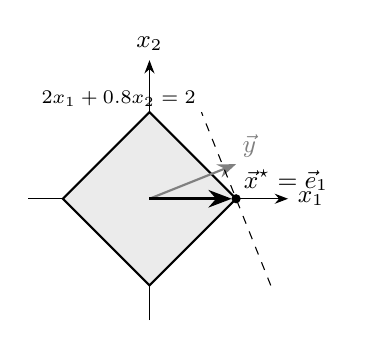
\begin{tikzpicture}[scale=1.1, >=Stealth]
    \draw[->] (-1.4,0) -- (1.6,0) node[right] {\small $x_1$};
    \draw[->] (0,-1.4) -- (0,1.6) node[above] {\small $x_2$};
    % Diamond
    \fill[black!8] (1,0) -- (0,1) -- (-1,0) -- (0,-1) -- cycle;
    \draw[thick] (1,0) -- (0,1) -- (-1,0) -- (0,-1) -- cycle;
    % y vector (2, 0.8), scaled to fit: show at (1.0, 0.4)
    \draw[->, thick, black!50] (0,0) -- (1.0, 0.4) node[above right=-2pt] {\small $\vec{y}$};
    % x* at right vertex (1,0) since y1 is largest
    \fill (1,0) circle (1.5pt);
    \draw[->, very thick] (0,0) -- (0.95,0);
    \node[above right=-1pt] at (1,0) {\small $\vec{x}^\star = \vec{e}_1$};
    % Supporting line: 2*x1 + 0.8*x2 = 2, tangent at (1,0)
    % At x1=1: 0.8*x2=0 => x2=0; at x2=1: x1=(2-0.8)/2=0.6
    % at x2=-1: x1=(2+0.8)/2=1.4
    \draw[thin, dashed] (1.4, -1.0) -- (0.6, 1.0)
        node[pos=1.0, above left=-2pt] {\scriptsize $2x_1+0.8x_2=2$};
\end{tikzpicture}
\end{center}

%------------------------------------------------------------------------------
\subsection{Case $p = \infty$: Cube Ball}
%------------------------------------------------------------------------------

\begin{example}[$p = \infty$]
Maximize $\vec{x}^\top \vec{y}$ subject to $\|\vec{x}\|_\infty \le 1$, with $\vec{y} = (-2, 3)^\top$.
\end{example}

The constraint $\|\vec{x}\|_\infty \le 1$ means each component satisfies $x_i \in [-1, 1]$. To maximize $\vec{x}^\top \vec{y} = \sum_i x_i y_i$, choose each $x_i$ independently to maximize $x_i y_i$:
\[
    x_i^\star = \sign(y_i)
\]

For $\vec{y} = (-2, 3)^\top$: $\vec{x}^\star = (-1, 1)^\top$, giving $\vec{x}^{\star\top} \vec{y} = (-1)(-2) + (1)(3) = 5 = |-2| + |3| = \|\vec{y}\|_1$.

\textbf{Formal proof.} For any $\vec{x}$ with $\|\vec{x}\|_\infty \le 1$:
\[
    \vec{x}^\top \vec{y} = \sum_{i=1}^{n} x_i y_i \le \sum_{i=1}^{n} |x_i| |y_i| \le \sum_{i=1}^{n} |y_i| = \|\vec{y}\|_1
\]

\begin{example}[Numerical: $p = \infty$]
Let $\vec{y} = (2, -5, 1)^\top$. Then $\vec{x}^\star = (1, -1, 1)^\top$, $\|\vec{x}^\star\|_\infty = 1$, and:
\[
    \vec{x}^{\star\top} \vec{y} = 2 + 5 + 1 = 8 = |2| + |-5| + |1| = \|\vec{y}\|_1 \checkmark
\]
\end{example}

\begin{tcolorbox}[colframe=black!50]
\textbf{Result:} $\displaystyle\max_{\|\vec{x}\|_\infty \le 1} \vec{x}^\top \vec{y} = \|\vec{y}\|_1$. The conjugate of the $\ell_\infty$ norm is the $\ell_1$ norm.
\end{tcolorbox}

\textit{Geometric meaning: The $\ell_\infty$-ball is a square. The best point is the corner whose signs match the signs of $\vec{y}$.}

\begin{center}
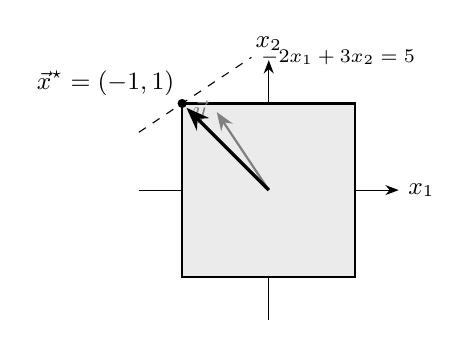
\begin{tikzpicture}[scale=1.1, >=Stealth]
    \draw[->] (-1.5,0) -- (1.5,0) node[right] {\small $x_1$};
    \draw[->] (0,-1.5) -- (0,1.5) node[above] {\small $x_2$};
    % Square
    \fill[black!8] (-1,-1) rectangle (1,1);
    \draw[thick] (-1,-1) rectangle (1,1);
    % y vector (-2,3), scaled to fit: show at (-0.6, 0.9)
    \draw[->, thick, black!50] (0,0) -- (-0.6,0.9) node[left] {\small $\vec{y}$};
    % x* at corner (-1,1) matching signs of y
    \fill (-1,1) circle (1.5pt);
    \draw[->, very thick] (0,0) -- (-0.95,0.95);
    \node[above left=-1pt] at (-1,1) {\small $\vec{x}^\star = (-1,1)$};
    % Supporting line: -2*x1 + 3*x2 = 5, tangent at (-1,1)
    % At x1=-1: 3*x2=3 => x2=1; at x1=-1.5: 3*x2=2 => x2=0.667
    \draw[thin, dashed] (-1.5, 0.667) -- (-0.2, 1.533)
        node[pos=1.0, right] {\scriptsize $-2x_1+3x_2=5$};
\end{tikzpicture}
\end{center}

%------------------------------------------------------------------------------
\subsection{General Maximizer for $1 < p < \infty$}
%------------------------------------------------------------------------------

For general $p \in (1, \infty)$ with conjugate exponent $q$ satisfying $\frac{1}{p} + \frac{1}{q} = 1$, the optimal solution is:

\begin{result}
\[
    x_i^\star = \frac{\sign(y_i) \, |y_i|^{q-1}}{\|\vec{y}\|_q^{q-1}}
\]
\end{result}

\textbf{Verification of feasibility} ($\|\vec{x}^\star\|_p = 1$). Using the identity $p(q-1) = q$:
\[
    \|\vec{x}^\star\|_p^p = \sum_{i=1}^{n} |x_i^\star|^p = \sum_{i=1}^{n} \frac{|y_i|^{p(q-1)}}{\|\vec{y}\|_q^{p(q-1)}} = \frac{1}{\|\vec{y}\|_q^q} \sum_{i=1}^{n} |y_i|^q = \frac{\|\vec{y}\|_q^q}{\|\vec{y}\|_q^q} = 1
\]

\textbf{Verification of optimality} ($\vec{x}^{\star\top} \vec{y} = \|\vec{y}\|_q$):
\[
    \vec{x}^{\star\top} \vec{y} = \sum_{i=1}^{n} \frac{\sign(y_i) \, |y_i|^{q-1}}{\|\vec{y}\|_q^{q-1}} \cdot y_i = \frac{1}{\|\vec{y}\|_q^{q-1}} \sum_{i=1}^{n} |y_i|^q = \frac{\|\vec{y}\|_q^q}{\|\vec{y}\|_q^{q-1}} = \|\vec{y}\|_q
\]

This matches the H\"{o}lder upper bound, confirming optimality for all $1 < p < \infty$.

\begin{tcolorbox}[colframe=black!50]
\textbf{Key identity used:} Since $\frac{1}{p} + \frac{1}{q} = 1$, we have $q = \frac{p}{p-1}$, so $q - 1 = \frac{1}{p-1}$ and $p(q-1) = \frac{p}{p-1} = q$.
\end{tcolorbox}

\begin{example}[Numerical: $p = 3$]
Let $p = 3$, so $q = \frac{3}{2}$. Let $\vec{y} = (1, 1)^\top$. Then $\|\vec{y}\|_{3/2} = (1 + 1)^{2/3} = 2^{2/3}$.

Using $q - 1 = \frac{1}{2}$, the maximizer is $x_i^\star = 1^{1/2} / (2^{2/3})^{1/2} = 2^{-1/3}$, so $\vec{x}^\star = 2^{-1/3}(1, 1)^\top$.

\textbf{Feasibility:} $\|\vec{x}^\star\|_3 = (2^{-1} + 2^{-1})^{1/3} = 1^{1/3} = 1$. $\checkmark$

\textbf{Optimality:} $\vec{x}^{\star\top} \vec{y} = 2 \cdot 2^{-1/3} = 2^{2/3} = \|\vec{y}\|_{3/2}$. $\checkmark$
\end{example}

%------------------------------------------------------------------------------
\subsection{The Dual Norm Pattern}
%------------------------------------------------------------------------------

The cases above reveal a beautiful pattern. In each case, optimizing over the $\ell_p$ ball yields the conjugate $\ell_q$ norm:

\begin{result}
\[
    \max_{\|\vec{x}\|_p \le 1} \vec{x}^\top \vec{y} = \|\vec{y}\|_q \quad \text{where } \frac{1}{p} + \frac{1}{q} = 1
\]
\end{result}

The norm $\|\cdot\|_q$ is called the \textbf{dual norm} of $\|\cdot\|_p$. H\"{o}lder's inequality provides the upper bound, and the explicit constructions above show the bound is tight for every $p \ge 1$.

\begin{center}
\begin{tabular}{ccc}
\toprule
$p$ & $q$ (conjugate) & Dual norm \\
\midrule
$1$ & $\infty$ & $\|\cdot\|_\infty$ \\
$2$ & $2$ & $\|\cdot\|_2$ \\
$\infty$ & $1$ & $\|\cdot\|_1$ \\
\bottomrule
\end{tabular}
\end{center}

\begin{center}
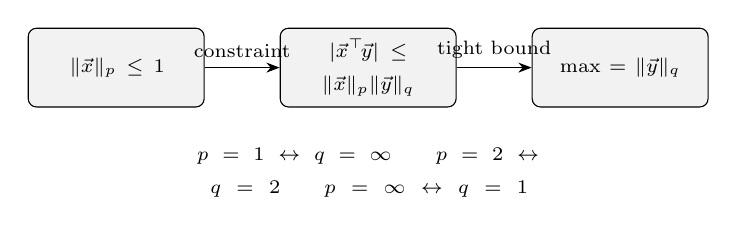
\begin{tikzpicture}[>=Stealth, every node/.style={align=center}]
    % Left box
    \node[draw, rounded corners=3pt, text width=2.0cm, minimum height=1.0cm, fill=black!5] (left) at (0,0)
        {\scriptsize $\|\vec{x}\|_p \le 1$};
    % Middle box
    \node[draw, rounded corners=3pt, text width=2.0cm, minimum height=1.0cm, fill=black!5] (mid) at (3.2,0)
        {\scriptsize $|\vec{x}^\top\!\vec{y}| \le \|\vec{x}\|_p \|\vec{y}\|_q$};
    % Right box
    \node[draw, rounded corners=3pt, text width=2.0cm, minimum height=1.0cm, fill=black!5] (right) at (6.4,0)
        {\scriptsize $\max = \|\vec{y}\|_q$};
    % Arrows
    \draw[->] (left) -- (mid) node[midway, above] {\scriptsize constraint};
    \draw[->] (mid) -- (right) node[midway, above] {\scriptsize tight bound};
    % Conjugate pairs below
    \node[below=0.4cm, text width=6cm] at (3.2, -0.5)
        {\scriptsize $p=1 \leftrightarrow q=\infty \quad\quad p=2 \leftrightarrow q=2 \quad\quad p=\infty \leftrightarrow q=1$};
\end{tikzpicture}
\end{center}

The $\ell_2$ norm is self-dual ($q = 2$ when $p = 2$), which is one reason it is so special.

%------------------------------------------------------------------------------
\subsection{Problem Solving Strategy: Separability}
%------------------------------------------------------------------------------

\begin{tcolorbox}
\textbf{Strategy (Separability).} When trying to simplify an optimization problem, check whether it decomposes into independent scalar problems. Solve each separately, then assemble the vector solution.
\end{tcolorbox}

This is the structure of the $p = \infty$ case. The constraint $\|\vec{x}\|_\infty \le 1$ means $-1 \le x_i \le 1$ for each component \emph{independently}, so the vector problem
\[
    \max_{\|\vec{x}\|_\infty \le 1} \sum_{i=1}^{n} x_i y_i
\]
decomposes into $n$ independent scalar problems $\max_{-1 \le x_i \le 1} x_i y_i$, each solved by $x_i^\star = \sign(y_i)$.

\begin{tcolorbox}[colframe=black!50]
\textbf{When to use this:} Separability applies when the constraint set is a Cartesian product of per-component constraints \emph{and} the objective is a sum of per-component terms. The $\ell_\infty$ ball is $[-1,1]^n$, so this works. The $\ell_1$ and $\ell_2$ balls couple the components, so separability does not apply.
\end{tcolorbox}

\begin{center}
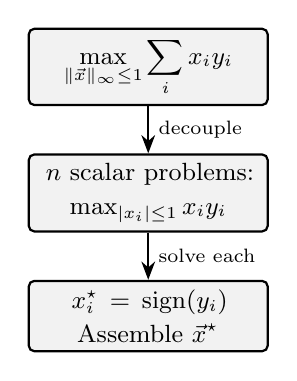
\begin{tikzpicture}[>=Stealth, node distance=0.6cm,
    box/.style={draw, thick, rounded corners=2pt, fill=black!5,
                minimum height=0.7cm, text width=2.8cm, align=center, font=\small}]
    \node[box] (vec) {$\displaystyle\max_{\|\vec{x}\|_\infty \le 1} \sum_i x_i y_i$};
    \node[box, below=of vec] (scalar) {$n$ scalar problems:\\[1pt] $\max_{|x_i|\le 1} x_i y_i$};
    \node[box, below=of scalar] (sol) {$x_i^\star = \sign(y_i)$\\[1pt] Assemble $\vec{x}^\star$};
    \draw[->, thick] (vec) -- node[right, font=\scriptsize] {decouple} (scalar);
    \draw[->, thick] (scalar) -- node[right, font=\scriptsize] {solve each} (sol);
\end{tikzpicture}
\end{center}

%------------------------------------------------------------------------------
\subsection{Problem Solving Strategy: Bound and Attain}
%------------------------------------------------------------------------------

\begin{tcolorbox}
\textbf{Strategy (Bound and Attain).} To solve an optimization problem:
\begin{enumerate}
    \item \textbf{Bound:} Use an inequality to establish an upper bound on the objective over all feasible points.
    \item \textbf{Attain:} Construct a specific feasible point that achieves the upper bound with equality.
\end{enumerate}
\end{tcolorbox}

This is the proof structure we used for the $p = 1$ case and the general dual norm result. First, H\"{o}lder gives the bound:
\[
    \vec{x}^\top \vec{y} \le \|\vec{x}\|_p \, \|\vec{y}\|_q \le \|\vec{y}\|_q
\]
Then we constructed an explicit $\vec{x}^\star$ achieving equality. Together, the two steps prove that the optimum is exactly $\|\vec{y}\|_q$.

\begin{tcolorbox}[colframe=black!50]
\textbf{Why this matters:} ``Bound and attain'' is one of the core proof templates in optimization. Many results in this course---including duality theory, minimax theorems, and optimality conditions---follow this two-step pattern.
\end{tcolorbox}

\begin{center}
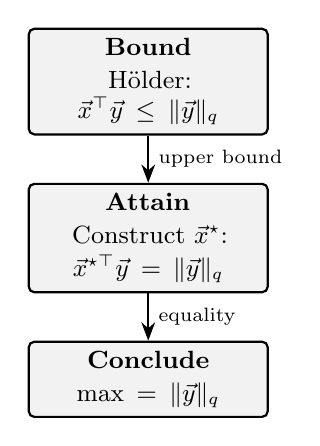
\begin{tikzpicture}[>=Stealth, node distance=0.6cm,
    box/.style={draw, thick, rounded corners=2pt, fill=black!5,
                minimum height=0.7cm, text width=2.8cm, align=center, font=\small}]
    \node[box] (bound) {\textbf{Bound}\\[1pt] H\"{o}lder: $\vec{x}^\top\vec{y} \le \|\vec{y}\|_q$};
    \node[box, below=of bound] (attain) {\textbf{Attain}\\[1pt] Construct $\vec{x}^\star$:\\[1pt] $\vec{x}^{\star\top}\vec{y} = \|\vec{y}\|_q$};
    \node[box, below=of attain] (opt) {\textbf{Conclude}\\[1pt] $\max = \|\vec{y}\|_q$};
    \draw[->, thick] (bound) -- node[right, font=\scriptsize] {upper bound} (attain);
    \draw[->, thick] (attain) -- node[right, font=\scriptsize] {equality} (opt);
\end{tikzpicture}
\end{center}

%==============================================================================
\section{Gram--Schmidt and QR Decomposition}
%==============================================================================

Given a set of linearly independent vectors $\{\vec{a}_1, \vec{a}_2, \ldots, \vec{a}_m\}$, the \textbf{Gram--Schmidt process} produces an orthonormal set $\{\vec{q}_1, \vec{q}_2, \ldots, \vec{q}_m\}$ spanning the same subspace.

%------------------------------------------------------------------------------
\subsection{The Gram--Schmidt Process}
%------------------------------------------------------------------------------

\textbf{Step 1: Normalize the first vector.}
\[
    \vec{q}_1 = \frac{\vec{a}_1}{\|\vec{a}_1\|_2}
\]

\textbf{Step 2: Orthogonalize and normalize $\vec{a}_2$.}

Project $\vec{a}_2$ onto $\vec{q}_1$ and subtract:
\[
    \vec{s}_2 = \vec{a}_2 - \langle \vec{a}_2, \vec{q}_1 \rangle \vec{q}_1
\]

The residual $\vec{s}_2$ is orthogonal to $\vec{q}_1$. Normalize:
\[
    \vec{q}_2 = \frac{\vec{s}_2}{\|\vec{s}_2\|_2}
\]

\textbf{Step 3: Orthogonalize and normalize $\vec{a}_3$.}

Project $\vec{a}_3$ onto $\vec{q}_1$ and $\vec{q}_2$, then subtract both:
\[
    \vec{s}_3 = \vec{a}_3 - \langle \vec{a}_3, \vec{q}_1 \rangle \vec{q}_1 - \langle \vec{a}_3, \vec{q}_2 \rangle \vec{q}_2
\]

Normalize: $\vec{q}_3 = \vec{s}_3 / \|\vec{s}_3\|_2$.

\textbf{General step $k$:} Subtract projections onto all previous $\vec{q}_i$:
\begin{result}
\[
    \vec{s}_k = \vec{a}_k - \sum_{i=1}^{k-1} \langle \vec{a}_k, \vec{q}_i \rangle \vec{q}_i, \qquad \vec{q}_k = \frac{\vec{s}_k}{\|\vec{s}_k\|_2}
\]
\end{result}

\textit{Geometric picture: orthogonalizing two vectors in $\RR^2$.}

\begin{center}
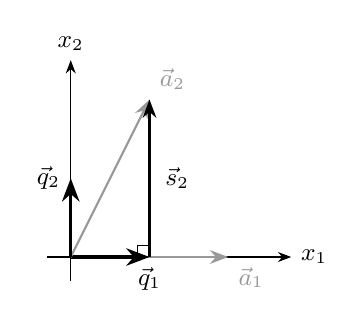
\begin{tikzpicture}[scale=1.0, >=Stealth]
    \draw[->] (-0.3,0) -- (2.8,0) node[right] {\small $x_1$};
    \draw[->] (0,-0.3) -- (0,2.5) node[above] {\small $x_2$};
    % a1 = (2,0) gray
    \draw[->, thick, black!40] (0,0) -- (2,0) node[below right] {\small $\vec{a}_1$};
    % q1 = (1,0) black, very thick
    \draw[->, very thick] (0,0) -- (1,0) node[below] {\small $\vec{q}_1$};
    % a2 = (1,2) gray
    \draw[->, thick, black!40] (0,0) -- (1,2) node[above right] {\small $\vec{a}_2$};
    % Dashed projection line from a2=(1,2) to proj=(1,0)
    \draw[dashed, thin, black!50] (1,2) -- (1,0);
    % Residual s2 from (1,0) to (1,2)
    \draw[->, thick] (1,0) -- (1,2) node[midway, right=2pt] {\small $\vec{s}_2$};
    % q2 = (0,1) black, very thick
    \draw[->, very thick] (0,0) -- (0,1) node[left] {\small $\vec{q}_2$};
    % Right-angle marker at (1,0)
    \draw[thin] (1,0.15) -- (0.85,0.15) -- (0.85,0);
\end{tikzpicture}
\end{center}

%------------------------------------------------------------------------------
\subsection{QR Decomposition}
%------------------------------------------------------------------------------

Gram--Schmidt gives us a matrix factorization. The key insight is that each original vector $\vec{a}_k$ can be written as a linear combination of the orthonormal vectors $\vec{q}_1, \ldots, \vec{q}_k$.

\textbf{Recovering $\vec{a}_k$ from $\vec{q}_k$.} By rearranging the Gram--Schmidt equations:

\textit{Column 1:} Since $\vec{q}_1 = \vec{a}_1 / \|\vec{a}_1\|_2$, we have
\[
    \vec{a}_1 = \|\vec{a}_1\|_2 \, \vec{q}_1
\]

\textit{Column 2:} Since $\vec{s}_2 = \vec{a}_2 - \langle \vec{a}_2, \vec{q}_1 \rangle \vec{q}_1$ and $\vec{q}_2 = \vec{s}_2 / \|\vec{s}_2\|_2$, we get $\vec{s}_2 = \|\vec{s}_2\|_2 \, \vec{q}_2$, so
\[
    \vec{a}_2 = \langle \vec{a}_2, \vec{q}_1 \rangle \vec{q}_1 + \|\vec{s}_2\|_2 \, \vec{q}_2
\]

\textit{Column 3:} Similarly,
\[
    \vec{a}_3 = \langle \vec{a}_3, \vec{q}_1 \rangle \vec{q}_1 + \langle \vec{a}_3, \vec{q}_2 \rangle \vec{q}_2 + \|\vec{s}_3\|_2 \, \vec{q}_3
\]

\textbf{Reading off the matrix $R$.} Write $A = [\vec{a}_1, \vec{a}_2, \ldots, \vec{a}_m]$ and $Q = [\vec{q}_1, \vec{q}_2, \ldots, \vec{q}_m]$. The column relations above become $A = QR$, where:

\begin{result}
\[
    A = QR, \qquad R = \begin{pmatrix}
        r_{11} & r_{12} & r_{13} & \cdots \\
        0 & r_{22} & r_{23} & \cdots \\
        0 & 0 & r_{33} & \cdots \\
        \vdots & \vdots & \vdots & \ddots
    \end{pmatrix}
\]
\end{result}

\textit{Schematic view of $A = QR$:}

\begin{center}
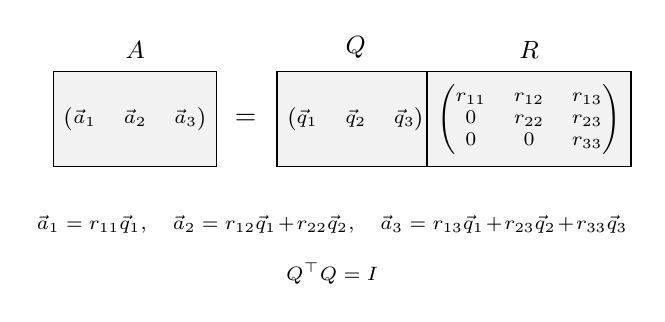
\begin{tikzpicture}[>=Stealth, every node/.style={align=center}]
    % A matrix
    \node[draw, minimum width=1.6cm, minimum height=1.2cm, fill=black!5] (A) at (0,0)
        {\scriptsize $\begin{pmatrix} \vec{a}_1 & \vec{a}_2 & \vec{a}_3 \end{pmatrix}$};
    \node[above=1pt] at (A.north) {\small $A$};
    % Equals sign
    \node at (1.4,0) {$=$};
    % Q matrix
    \node[draw, minimum width=1.6cm, minimum height=1.2cm, fill=black!5] (Q) at (2.8,0)
        {\scriptsize $\begin{pmatrix} \vec{q}_1 & \vec{q}_2 & \vec{q}_3 \end{pmatrix}$};
    \node[above=1pt] at (Q.north) {\small $Q$};
    % R matrix
    \node[draw, minimum width=1.6cm, minimum height=1.2cm, fill=black!5] (R) at (5.0,0)
        {\scriptsize $\begin{pmatrix} r_{11} & r_{12} & r_{13} \\ 0 & r_{22} & r_{23} \\ 0 & 0 & r_{33} \end{pmatrix}$};
    \node[above=1pt] at (R.north) {\small $R$};
    % Column expansions below
    \node[below=0.5cm, text width=7.5cm] at (2.5, -0.6)
        {\scriptsize $\vec{a}_1 = r_{11}\vec{q}_1, \quad
         \vec{a}_2 = r_{12}\vec{q}_1 + r_{22}\vec{q}_2, \quad
         \vec{a}_3 = r_{13}\vec{q}_1 + r_{23}\vec{q}_2 + r_{33}\vec{q}_3$};
    % Q^T Q = I note
    \node[below=1.1cm] at (2.5, -0.6) {\scriptsize $Q^\top Q = I$};
\end{tikzpicture}
\end{center}

The entries of the upper-triangular matrix $R$ come directly from the Gram--Schmidt process:
\begin{itemize}
    \item \textbf{Diagonal entries:} $r_{kk} = \|\vec{s}_k\|_2$ \quad (normalization factors)
    \item \textbf{Off-diagonal entries:} $r_{jk} = \vec{q}_j^\top \vec{a}_k$ for $j < k$ \quad (projection coefficients)
\end{itemize}

The matrix $Q$ has \textbf{orthonormal columns}, meaning $Q^\top Q = I$. This follows because $\vec{q}_i^\top \vec{q}_j = 0$ for $i \ne j$ (orthogonality) and $\vec{q}_i^\top \vec{q}_i = 1$ (normalization).

\begin{tcolorbox}[colframe=black!50]
\textbf{Why QR matters:} The QR decomposition converts the normal equations $A^\top A \vec{x} = A^\top \vec{y}$ into the simpler system $R\vec{x} = Q^\top \vec{y}$, which is easy to solve by back-substitution. This is numerically more stable than computing $A^\top A$ directly.

\medskip

\textit{Derivation:} Since $A = QR$ and $Q^\top Q = I$, we have $A^\top A = R^\top R$ and $A^\top \vec{y} = R^\top Q^\top \vec{y}$. The normal equations become $R^\top R \vec{x} = R^\top Q^\top \vec{y}$. Since $R$ is invertible (each $r_{kk} > 0$), cancel $R^\top$ to get $R\vec{x} = Q^\top \vec{y}$.
\end{tcolorbox}

%------------------------------------------------------------------------------
\subsection{Big Picture}
%------------------------------------------------------------------------------

This lecture developed two themes that reappear throughout the course.

\textbf{Norms and dual norms.} Optimizing a linear function over a norm ball reveals the dual norm:
\begin{result}
\[
    \max_{\|\vec{x}\|_p \le 1} \vec{x}^\top \vec{y} = \|\vec{y}\|_q, \qquad \frac{1}{p} + \frac{1}{q} = 1
\]
\end{result}

The three key dual pairs are:
\begin{itemize}
    \item $\ell_1 \leftrightarrow \ell_\infty$: the dual of the $\ell_1$ norm is the $\ell_\infty$ norm
    \item $\ell_2 \leftrightarrow \ell_2$: the $\ell_2$ norm is self-dual
    \item $\ell_\infty \leftrightarrow \ell_1$: the dual of the $\ell_\infty$ norm is the $\ell_1$ norm
\end{itemize}

\textbf{Orthogonality and QR.} The Gram--Schmidt process converts any set of linearly independent vectors into an orthonormal set spanning the same subspace. Recording the coefficients in a matrix yields the QR decomposition $A = QR$, which provides a numerically stable route to solving least-squares problems.

%==============================================================================

\vfill

\section*{Key Takeaways}

\begin{enumerate}
    \item \textbf{A norm measures vector size:} it must satisfy non-negativity, the triangle inequality, and absolute homogeneity.
    \item \textbf{The $\ell_p$ norms} form a family parameterized by $p$: $p=1$ (sum of absolute values), $p=2$ (Euclidean), $p=\infty$ (max component).
    \item \textbf{Cauchy--Schwarz} bounds the inner product: $|\vec{x}^\top \vec{y}| \le \|\vec{x}\|_2 \|\vec{y}\|_2$. H\"{o}lder generalizes this to all $\ell_p$ norms.
    \item \textbf{Minkowski's inequality} ($\|\vec{u}+\vec{v}\|_p \le \|\vec{u}\|_p + \|\vec{v}\|_p$) proves the triangle inequality for $\ell_p$ norms via H\"{o}lder.
    \item \textbf{Norm balls} visualize constraints: diamond ($p=1$), circle ($p=2$), square ($p=\infty$).
    \item \textbf{Dual norm pattern:} $\max_{\|\vec{x}\|_p \le 1} \vec{x}^\top \vec{y} = \|\vec{y}\|_q$ where $\frac{1}{p} + \frac{1}{q} = 1$. The general maximizer is $x_i^\star = \sign(y_i)|y_i|^{q-1}/\|\vec{y}\|_q^{q-1}$.
    \item \textbf{Two proof strategies:} \emph{Separability} (decouple into independent scalar problems) and \emph{Bound-and-Attain} (establish an upper bound via an inequality, then construct a feasible point achieving it).
    \item \textbf{Gram--Schmidt} converts linearly independent vectors to an orthonormal basis, yielding the QR decomposition $A = QR$.
\end{enumerate}

\end{document}
